\documentclass{article}
\usepackage[utf8]{inputenc}
\usepackage{graphicx}
\usepackage{geometry}
\usepackage{amsmath}
\usepackage{amsfonts}
\usepackage{float}
\usepackage{caption}
\usepackage{subcaption}
\usepackage{enumitem}

\geometry{left=25mm, top=25mm, right=25mm, bottom=25mm}

\title{PHY407 Lab 7}
\author{Pierino Zindel (1002429703) and Hayden Johnson (1002103537)}
\date{October 26, 2018}

\begin{document}

\maketitle

\noindent \textbf{Distribution of work:} Question 1 was completed by Pierino. Question 2 was completed by Hayden.

\section{Return of the Space Garbage}

\section{The Hydrogen Atom}

\subsection{Part b)}

We seek to use our program to compute the energies of the ground state and the first excited state (for $l=0$ and $l=1$), and observe the effects of changing various parameters on the accuracy of the computation.

The computed values of the energy for the first two excited states, along with the theoretical values, are displayed in table \ref{tab:2b_i}. These values were computed using the suggested parameter values of $h=0.002a$, $r_\infty=20a$ (where $a$ is the Bohr radius), and a target accuracy of $e/1000$, and we can see that the agreement with the theoretical values is quite good for $n=2, l=1$, is okay for $n=2, l=0$ and $n=1, l=0$.

\begin{table}[H]
	\centering
	\caption{Numerically calculated energy values of the ground state and first excited state of the hydrogen atom, along with the theoretical values. Program used suggested parameter values of $h=0.002a$, $r_\infty=20a$, and a target accuracy of $e/1000$.}
	\label{tab:2b_i}
	\begin{tabular}{c|c|c|c}
		$n$ & $l$ & Calculated $E$ (eV)  & Literature $E$ (eV) \\
		\hline
		1 & 0 & -13.5004889817 & -13.605693009 \\
		2 & 0 & -3.3878669497 & -3.40142325225 \\
		2 & 1 & -3.40127671989 & -3.40142325225 \\
	\end{tabular}
\end{table}

In table \ref{tab:2b_ii} we display the calculated values of the energy for the first three states for three different values of $r_\infty$ with fixed step size $h=0.002a$ and target accuracy of $e/1000$. As can be seen from the table, increasing the value of $r_\infty$ improves the accuracy of the solution in all cases, although the extent to which it does this depends on the particular energy level and angular momentum value, and in some cases (i.e. $n=1, l=0$ the observed improvements were negligible.

\begin{table}[H]
	\centering
	\caption{Numerically calculated energy values of the ground state and first excited state of the hydrogen atom, along with the theoretical values, for different values of $r_\infty$ with $h=0.002a$ and a target accuracy of $e/1000$.}
	\label{tab:2b_ii}
	\begin{tabular}{c|c|c|c|c|c}
		$n$ & $l$ & $r_\infty=10a$ &  $r_\infty=20a$ & $r_\infty=40a$ & Literature $E$ (eV) \\
		\hline
		1 & 0 & -13.5004703237 & -13.5004889817 & -13.5004917637 & -13.605693009 \\
		2 & 0 & -3.05116418764 & -3.3878669497 & -3.38822466074 &  -3.40142325225 \\
		2 & 1 & -3.23433299007 & -3.40127671989 & -3.40142286517 & -3.40142325225 \\
	\end{tabular}
\end{table}

In table \ref{tab:2b_iii} we display the calculated values of the energy for the first three states for three different values of $h$ with fixed $r_\infty=20a$ and target accuracy of $e/1000$. As can be seen from the table, the accuracy of the calculations invariably increases with a smaller step size, and this improvement seems to be better than that for an increase in the value of $r_\infty$, although it is difficult to compare these two things given that the size of the variations tested is different, and itself difficult to compare. 

\begin{table}[H]
	\centering
	\caption{Numerically calculated energy values of the ground state and first excited state of the hydrogen atom, along with the theoretical values, for different values of $h$ with $r_\infty=20a$ and a target accuracy of $e/1000$.}
	\label{tab:2b_iii}
	\begin{tabular}{c|c|c|c|c|c}
		$n$ & $l$ & $h = 0.02a$ & $h = 0.002a$ & $h = 0.0002a$ & Literature $E$ (eV) \\
		\hline
		1 & 0 & -12.7092157518 & -13.5004889817 & -13.5949027472 & -13.605693009 \\
		2 & 0 & -3.28576534849 & -3.3878669497 & -3.39972201792 & -3.40142325225 \\
		2 & 1 & -3.40126355429 & -3.40127671989 & -3.40127673348 & -3.40142325225 \\
	\end{tabular}
\end{table}

In table \ref{tab:2b_iiii} we display the calculated values of the energy for the first three states for three different values of the target accuracy and with $h=0.002a$ and $r_\infty=20a$. As can be seen from the table, changing the target accuracy does not seem to have a very big effect on the accuracy of the calculation. This seems surprising, but makes sense if we consider that the accuracy we are specifying is simply requiring the solution to get closer to the value to which it is converging, and if it is converging to the incorrect value then changing the ``accuracy'' will not actually make it more accurate.

\begin{table}[H]
	\centering
	\caption{Numerically calculated energy values of the ground state and first excited state of the hydrogen atom, along with the theoretical values, for different target accuracies with $h=0.002a$ and $r_\infty=20a$.}
	\label{tab:2b_iiii}
	\begin{tabular}{c|c|c|c|c|c}
		$n$ & $l$ & target$=e/100$ & target$=e/1000$ & target$=e/10000$ & Literature $E$ (eV) \\
		\hline
		1 & 0 & -13.5009218107 & -13.5004889875 & -13.5004919696 & -13.605693009 \\
		2 & 0 & -3.38784656151 & -3.38786638765 & -3.38786638765 & -3.40142325225 \\
		2 & 1 & -3.40120743963 & -3.40127648895 & -3.40127648895 & -3.40142325225 \\
	\end{tabular}
\end{table}

\subsection{Part d)}

We seek to produce plots of the normalized computed wavefunctions $R(r)$ for each of the energy levels from the previous section, and compare the graphs of the functions to those of the theoretical solutions to the differential equation.

Plots of the eigenfunctions for all three sets of $n$ and $l$ values are shown in figures \ref{fig:q2_d_n=1_l=0}-\ref{fig:q2_d_n=2_l=1}. In light of the discussion in part b), we used parameter values of $h=0.0002a$, $r_\infty=20a$, and target accuracy of  $e/1000$ to compute the wavefunctions. In all figures, both the computed and theoretical wavefunctions have been normalized. As can be seen from the figures, the overall agreement between the computed and theoretical functions on the breadth of the domain is very good; the only discernible discrepancies occur at the endpoint $r=0$.

In the case of both $n=1, l=0$ (figure \ref{fig:q2_d_n=1_l=0}) and $n=2, l=0$ (figure \ref{fig:q2_d_n=2_l=0}), we see that the theoretical wavefunction increases to infinity at r=0. However, we required the boundary condition that $R(0) = 0$ in the numerical solution, so the numerical solution satisfies this condition and then quickly jumps up to match the theoretical value and follows it pretty much exactly over the rest of the domain, with no visible discrepancies. Thus, ignoring this one predictable error of the numerical method, the shape and zero crossings of the numerically computed wave functions, for the tested energy levels, agree very well with those of the theoretical/analytically determined wave functions.

Note that in the case of $n=2, l=1$, displayed in figure \ref{fig:q2_d_n=2_l=1}, the wavefunction does actually satisfy our imposed boundary condition of $R(0) = 0$, and we see that the computed and analytic wavefunctions agree very well over the whole domain, as we would expect them to.

\begin{figure}[H]
	\centering
	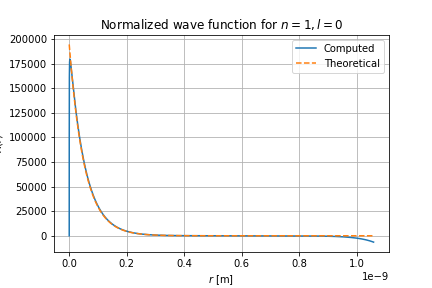
\includegraphics[width=0.8\textwidth]{../images/q2_d_n=1_l=0.png}
	\caption{Plot of computed and theoretical normalized wavefunction $R(r)$ for $n=1, l=0$.}
	\label{fig:q2_d_n=1_l=0}
\end{figure}

\begin{figure}[H]
	\centering
	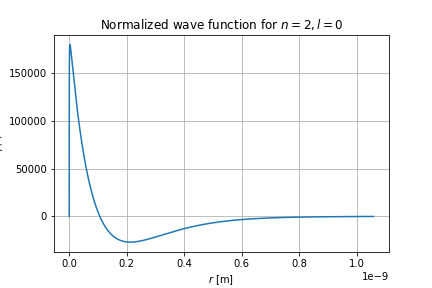
\includegraphics[width=0.8\textwidth]{../images/q2_d_n=2_l=0.png}
	\caption{Plot of computed and theoretical normalized wavefunction $R(r)$ for $n=2, l=0$.}
	\label{fig:q2_d_n=2_l=0}
\end{figure}

\begin{figure}[H]
	\centering
	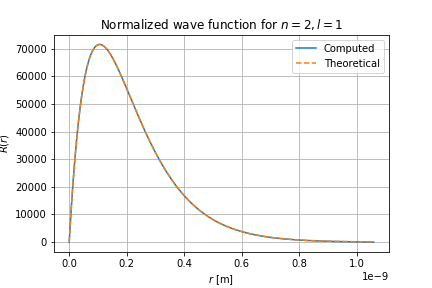
\includegraphics[width=0.8\textwidth]{../images/q2_d_n=2_l=1.png}
	\caption{Plot of computed and theoretical normalized wavefunction $R(r)$ for $n=2, l=1$.}
	\label{fig:q2_d_n=2_l=1}
\end{figure}

\end{document}
